% LaTeX Article Template - customizing header and footer
\documentclass [11point]{article}

% Set left margin - The default is 1 inch, so the following 
% command sets a 1.25-inch left margin.

\setlength{\oddsidemargin}{0.25in}
% Set width of the text - What is left will be the right margin.
% In this case, right margin is 8.5in - 1.25in - 6in = 1.25in.
\setlength{\textwidth}{6.5in}

% Set top margin - The default is 1 inch, so the following 
% command sets a 0.75-inch top margin.
%\setlength{\topmargin}{-0.25in}

% Set height of the header
\setlength{\headheight}{0.3in}

% Set vertical distance between the header and the text
\setlength{\headsep}{0.2in}

% Set height of the text
\setlength{\textheight}{9in}

% Set vertical distance between the text and the
% bottom of footer
\setlength{\footskip}{0.1in}

\parindent0pt
\def \rn { {\rm I} \!\! \! {\rm R}^n }

\usepackage{graphicx,url}
\usepackage{amssymb}
\usepackage{amsthm}
\usepackage{amsmath,color}


% Set the beginning of a LaTeX document
\begin{document}

% Redefine "plain" pagestyle
\makeatletter	   % `@' is now a normal "letter' for LaTeX
\renewcommand{\ps@plain}{%
     \renewcommand{\@oddhead}{\textrm{\small {\it DSC Prelim Exam -- Summer 2011}}\hfil\textrm{\thepage}}% 
     \renewcommand{\@evenhead}{\@oddhead}%
     \renewcommand{\@oddfoot}{}% empty footer
     \renewcommand{\@evenfoot}{\@oddfoot}}
\makeatother     % `@' is restored as a "non-letter" character

\title{
\hrule 
\bigskip
Department of Scientific Computing\\
\textbf{Written Preliminary Examination} \\
Summer 2011 \\
}         % Enter your title between curly braces
\author{}        % Enter your name between curly braces
\date{July 6, 2011}          % Enter your date or \today between curly braces
\maketitle

% Set to use the "plain" pagestyle
\pagestyle{plain}

\hrule 
\bigskip
\textit{Instructions:}

\bigskip

\begin{itemize}
\item Solve only 10 of the 11 questions as completely as you can. 

\item All questions are weighted equally.

\item All parts of a question are weighted equally unless stated otherwise.

\item If you use web sources, please list them clearly.

\item The exam is due back to Dr. Sachin Shanbhag no later than 1:00 pm on Saturday, July 9, 2011; no exceptions allowed. If you finish ahead to time, slip it under the door to his office.

\item If you have any questions related to this exam as you work on it, please send an e-mail to the person responsible, \textit{and} Dr. Sachin Shanbhag (sshanbhag at fsu dot edu). The person responsible is listed at the beginning of each question.

\item Write your Student ID on each of your answer sheets. Do not write your name on your answer sheets. When turning in your exam, include a cover page with your name and Student ID.

\end{itemize}

\medskip
\hrule

\pagebreak
\hrule 
\medskip
1. \textit{Linear Algebra} (Dr. Peterson)
\bigskip

One way to generate a stationary iterative method for the solution of $A \vec x = \vec b$ is to split $A$ as $A=A_1+A_2$ to obtain the following iteration.
\smallskip
Given $\vec x^0$; for $k=0,1,2,\ldots$ find $\vec x^{k+1}$ by solving the linear system
$$A_1 \vec x^{k+1} = -A_2 \vec x ^k + \vec b \,. $$
Here $P=-A_1^{-1}A_2$ is called the {\it iteration matrix} for the method where of course $A_1$ is invertible.\medskip

a.\quad  The component form of the standard Gauss-Seidel method is
$$ x^{k+1}_i = {1 \over a_{ii} } \big( b_i - \sum_{j<i} a_{ij}x_j^{k+1} - \sum_{j>i} a_{ij}x_j^{k }\big) \quad i=1,2, \ldots, n$$
where $a_{ij}$ denotes the $(i,j)$ entry of the $n \times n$ matrix $A$.  Derive $A_1$ and $A_2$ for this standard Gauss-Seidel method. \medskip

b.\quad Unlike the Jacobi method, in the standard Gauss-Seidel method the ordering of the unknowns is important.  In the method of (a) we begin by updating the   first coordinate of our iterate.  We can also begin with the {\it last} component of the iterate (i.e., update $x_n^{k+1}$ first).  Derive the matrix and component form of this modified Gauss-Seidel method. \medskip

c.\quad    An obvious extension of the standard Gauss-Seidel method is at each iteration to  perform two updates; in the first we start with the first component of $\vec x^{k+1}$ (as in the standard Gauss-Seidel given in (a)) and create say $\vec y^{k+1}$ and then    do a second update where we start  with the last component,  i.e., using your method of (b) starting with $\vec y^{k+1}$ to obtain  $  \vec x^{k+1}$. Obtain the iteration matrix $P$ for this method. \medskip

d.\quad  Use your algorithm in (c) to   obtain $\vec x^1, \vec x^2$ for the linear system $A \vec x = \vec b$ where
$$ A =\begin{pmatrix} \hfill 10 & \hfill  -1 & \hfill  0 \cr  \hfill -1 & \hfill 10 & \hfill -2 \cr  \hfill 0 & \hfill  -2 & \hfill 10 \end{pmatrix}  \qquad \vec b= \begin{pmatrix} 9 \cr 7 \cr 6 \end{pmatrix} \qquad \vec x^0 = \begin{pmatrix} 0\cr 0 \cr 0 \end{pmatrix} $$
\medskip

e.\quad  If your original matrix $A$ is symmetric and positive definite, then prove that your iteration matrix $P$ in (c) is also symmetric and positive definite.  

\bigskip
\hrule \medskip


\pagebreak
\hrule 
\medskip
2. \textit{Partial Differential Equations} (Dr. Peterson)
\bigskip

a.\quad  Let $\Omega$ be a bounded domain in $R^2$ with boundary $\Gamma = \Gamma_1 \cup \Gamma_2$ where $\Gamma_1 \cap \Gamma_2=\emptyset$.  Consider the following  PDE and boundary conditions for $u(x,y )$
$$-\Delta u +uu_x = f(x,y)  \quad (x,y) \in \Omega$$
$$ u=0 \quad \mbox{on $\Gamma_1$} \qquad \frac{\partial u}{\partial n} = 4 \quad \mbox{on $\Gamma_2$}$$
and the weak formulation
$$ \mbox{Seek $u \in \hat H^1$ satisfying} \hskip3in $$
$$ \int_\Omega \nabla u \cdot \nabla v + \int_\Omega u u_x v = \int_\Omega f v +4\int_{\Gamma_2} v \quad \forall v \in \hat H^1$$
where $\hat H^1$ is all functions that are zero on $\Gamma_1$ and which possess one weak derivative.  Here $\Delta u = u_{xx}+u_{yy}$ and $\partial u/\partial n$ denotes the derivative of $u$ in the direction of the unit outer normal, i.e., $\nabla u \cdot \vec n$.    \smallskip
Show that if $u$ satisfies the classical boundary value problem then it satisfies the weak problem.  Then show that if $u$ is a sufficiently smooth solution to the weak problem, then it satisfies the PDE and the boundary conditions. \medskip

 
b.\quad  Now let $w=w(x,t)$ and consider the initial boundary value problem
$$ w_t - w_{xx} = f(x,t) \quad 0 \le x \le 2, \quad t>0 $$
$$ w(0,t)=w(2,t) = 0 \quad t>0 $$
$$ w(x,0) = w_0 \quad  0 \le x \le 2$$
Write down an {\it implicit}   finite difference scheme for this problem which is {\it second order in space and time}.  Then show that at a fixed time, we are required to solve a linear system $A \vec w = \vec f$ and explicitly give $A$ and $\vec f$.  
\medskip

c.\quad Let $w(x,t)$.  Derive a finite difference approximation to $w_{xxx}(x,t)$ using the values $w(x,t)$, $w(x+h,t)$, $w(x-h,t)$ and $w(x+2h,t)$.  Determine the truncation error for your approximation.  

\bigskip
\hrule 

\pagebreak
\hrule 
\medskip
3. \textit{Constrained Optimization} (Dr. Navon)
\bigskip

Consider the $L_1$ exact penalty method for the constrained optimization  problem
$$ \min f(x),$$
$${\it s.t. }
\left. \begin{array}{c}
    g_i(x)=0,~i\in {\cal E} \\g_i(x)\geq 0, ~i\in I.  \end{array} \right.$$

We are assuming that $f$ and constraint functions $g_i$ are continuous.

Consider the penalty function:
$$\pi_{\rho}(x)=f(x)+\rho\sum_{i\in \cal E}|g_i(x)|-\rho\sum_{i\in I} \min(0,g_i(x)).$$

Apply it to the problem
$$ \min f(x)=\frac{1}{2}(x_1-x_2)^2 +\frac{1}{2}x_2^2,$$
$${\it s.t. }~~ x_1\geq 1.$$

Please derive the function $\pi_{\rho}(x)$, then show that for any $\rho>\frac{1}{2}$, $x_1=1$ is the minimizer of the function $f$ - and that this yields $x_2=\frac{1}{2}$.

Hence for any $\rho >\frac{1}{2}$, solution $x^*$ is also a minimizer of the penalty function $\pi_{\rho}(x)$.\bigskip

\textit{Hint}: The function $\pi_{\rho}(x)$ is not differentiable when $x_1=1$.


\bigskip 
\hrule

\pagebreak
\hrule
\medskip
4. \textit{Unconstrained Optimization} (Dr. Navon)
\bigskip

Consider the Davidon-Fletcher-Powell (DFP)
Q-N method for
$$f(x_1,x_2) = x_1-x_2 +2x_1^2 +2x_1x_2 +x_2^2 $$
with starting point $(0,0)^T$. The initial approximation
for the Hessian is
the unit matrix$$H_1 = \left[ \begin{array}{cc}
  1 & 0  \\
  0 & 1   \end{array} \right]
$$
a.\quad Show that the first search direction $d_1$ is the same as the steepest-descent direction $-\nabla f(x_1) $.
\medskip

b.\quad Obtain minimizing step-length $\lambda ^{\ast} _1$ along $d_1$,
update matrix $H_1$ and compute one full DFP iteration. Compute
$H_2$ and the new search direction $d_2 = -H_2 \nabla f(x_2) $
\medskip

Find minimizing step-length $\lambda ^{\ast} _2$ along $d_2$ by minimizing
$$f(x_2 + \lambda _2 d_2 ) $$
and obtain $x_3$.

\medskip

Show that this point $x_3$ is the optimum by showing
that $\nabla f(x_3) =(0,0)^T$.

\bigskip
\textit{Hint}: the DFP Q-N update is
$$H_{k+1} = H_k + \frac{p_kp_k^T}{p_k^Ty_k} -\frac{(H_ky_k)(H_ky_k)^T}{y_k^TH_ky_k}. $$


\bigskip 
\hrule 



\pagebreak
\hrule 
\medskip
5. \textit{Parallel Programming} AMB
\bigskip

Consider the following C++ program:

\begin{verbatim}
float prefixSum(float* x, int size) {
     float sum = 0;
     for( int i=0; i< size; i++){
          sum = sum + x[i];
     }
     return sum;
}
\end{verbatim}

\medskip

a.\quad Explain why the loop inside the \texttt{prefixSum} function cannot be parallelized as it is. Modify this loop and make a parallel version of it using pseudo code. In your algorithm show what loops are executed in parallel, and which variables are private or shared. You can assume the size of the vector \texttt{x} is a power of two.\medskip

b.\quad Describe the theoretical speedup of your algorithm. \medskip

\bigskip 
\hrule 

\pagebreak
\hrule 
\medskip
6. \textit{Datastructures} (Dr. Wang)
\bigskip

Suppose a simple closed surface divides the 3D space into two parts: inside and outside. Consider an unstructured triangular mesh of this closed surface: one array of integers \texttt{tri(nTri, 3)} that contains the indexes of the three vertices belonging to each of the \texttt{nTri} triangles, and one array of real numbers \texttt{node(nVert, 3)} that contains the positions of the \texttt{nVert} vertices.\medskip

We wish to compute the unit normal vectors uniformly towards inside or outside for each triangle with the least possible cost.\medskip

a.\quad In order to complete this task, you may need to reorganize the data with a datastructure. If you do, please make a detailed
description of your datastructure, and write the pseudocode used to generate the new data.\medskip

b.\quad Write a pseudocode that implements your algorithm to compute the required unit normal vectors based on your datastructure.\medskip

c.\quad In the most common case, what is the total asymptotic cost of your algorithm?


\bigskip
\hrule 


\pagebreak
\hrule 
\medskip
7. \textit{Linear Algebra} (Dr. Wang)
\bigskip

Suppose $A$ is a nonsingular $n \times n$ matrix. We would like to solve the system:
$$
\left[
\begin{array}{rr}
A & g \\
h^T & \alpha
\end{array} \right]
\left[
\begin{array}{r}
x \\
\mu
\end{array} \right]=
\left[
\begin{array}{rr}
b \\
\beta
\end{array} \right].
$$
where $\alpha, \beta$ are real numbers and $h, g$ and $b$ are
n-dimensional vectors. The unknowns are vector $x$ and real number
$\mu$.\medskip

In general, we cannot solve the system as fast as $O(n)$ flops. But let us say that we already know the solutions to the linear systems $Az=b$ and $Ay=g$.\medskip

a.\quad With the help of $z, y$, please show how to solve the system in $O(n)$ flops.\medskip

b.\quad Write down your algorithm in pseudo code.

\bigskip
\hrule 

\pagebreak
\hrule 
\medskip
8. \textit{Approximation} (Dr. Shanbhag)
\bigskip

We want to approximate the function $$ u(r) = \frac{1}{r^{12}} - \frac{1}{r^{6}},$$ over the range $0.9 \leq r \leq 2.0$.\medskip

a.\quad Using Chebyshev polynomials as a basis, find a tenth order polynomial approximation of the form: $$p_{10}(r) = \sum_{i=0}^{10} a_i T_i(\alpha r + \beta),$$ where $\alpha$ and $\beta$ are constants needed to transform the domain from $[0.9, 2.0]$ to $[-1, 1]$, and $a_i$ are the weights associated with $T_i$. You may use either ``interpolated" or ``truncated" Chebyshev series. Report the approximate $p_{10}(r)$, and a present a plot of the approximate and actual function over the domain $0.9 \leq r \leq 2.0$. (85 points)\medskip

b.\quad Estimate the $L_{2}$ norm for the approximate function. (15 points)

\bigskip
\hrule 




\pagebreak
\hrule 
\medskip
9. \textit{Gaussian Quadrature} (Dr. Shanbhag)
\bigskip

We are interested in developing quadrature rules for integrals of the form: $$ I = \int_0^{10} e^{-x} f(x) dx.$$\medskip

a.\quad Find the first three ($i$=0, 1, and 2) \textit{orthonormal} polynomials $P_i(x)$, with weight function $w(x) = e^{-x}$, and range [0, 10]. (60 points)\medskip

b.\quad Find the roots $x_1$ and $x_2$ of the polynomial $P_2(x)$. (10 points)\medskip

c.\quad Develop a 2-point quadrature rule $I \approx w_1 f(x_1) + w_2 f(x_2)$. Compare with the corresponding Gauss-Laguerre quadrature rule. (30 points) \medskip

\bigskip
\hrule 




\pagebreak
\hrule 
\medskip
10. \textit{Ordinary Differential Equations} (Dr. Erlebacher)
\bigskip

Consider the system of differential equations for $Q=(x(t),y(t))$:
\begin{eqnarray}
\frac{dx}{dt} &=& a x + b y \nonumber \\\frac{dy}{dt} &=& c x + d y  \nonumber\end{eqnarray}
Initial conditions are $x_0 = x(0) = 1$ and $y_0 = y(0) = -2$. Let $h=\Delta t$ be the numerical
time step.\medskip

a. \quad Choose non-zero values of the parameters $a$, $b$, $c$, $d$ such that the analytical solution to the differential equation has decaying solutions. (10 points) \medskip

b. \quad Derive a first order numerical algorithm using Taylor series. Show all steps of your derivation. (15 points) \medskip

c. \quad Derive a second order numerical algorithm using Taylor series. Show all steps of your derivation. (15 points) \medskip

d. \quad Derive a third order numerical algorithm using numerical integration formulas. Show all steps of your derivation. (15 points) \medskip

e. \quad Implement these three approaches numerically and solve the system of equations for $t=0$ to $t=1$ for a range of time steps ranging from $h=10^{-4}$ to $h=10^{-1}$ by increments of 10. Include the source code. Choose any language for coding. (20 points) \medskip

f. \quad Compute numerically the accuracy of the solution by comparing the numerical solution to the exact solution of the system of equations. Verify that the accuracy of the three algorithms are first, second and third order accurate. Present plots of the logarithm of the L2 norm of the error vector as a function of time for the different time steps. (15 points) \medskip

g. \quad What are the conditions on $a,b,c,d$ that lead to instability in the exact solution? (10 points)


\bigskip
\hrule 

\pagebreak
\hrule 
\medskip
11. \textit{Statistics and Random Processes} (Dr. Beerli)
\bigskip

A dataset contains heights of fictitious eagles that have a sexual dimorphism: females are considerably larger than males. The data can be downloaded from \url{http://people.sc.fsu.edu/~beerli/eagle.txt} (also see below). The data does not contain any information about the sex of the individuals. We also assume that the standard deviations of the height in males and females is the same and known from some breeding study ($\sigma=100$).\medskip

Task:
\begin{itemize}
\item {\bf Assign (and show) a probability of being female to every bird in the sample [the data is ordered from smallest to tallest]}.
\item {\bf Give the parameter values for the mixture model: $p, \mu_1, \mu_2$}
\item {\bf Show your program and thoughts}.
\end{itemize}
Use this mixture model with parameters $p$, $\mu_1$, and $\mu_2$, the standard deviations are fixed at $\sigma_1=\sigma_2=100$: 
$$
{\rm Prob}(x_i | p, \mu_1,\mu_2,\sigma_1=100,\sigma_2=100) = (1-p) \frac{1}{\sqrt{2\pi} \sigma_1} e^{-\frac{(x_i-\mu_1)^2}{2 \sigma_1^2}} + p \frac{1}{\sqrt{2\pi} \sigma_2} e^{-\frac{(x_i-\mu_2)^2}{2 \sigma_2^2}}
$$
and estimate the distribution parameters. This could be done either with a least-square method, a Bayesian approach (using MC or MCMC), or an expectation/maximization approach. Pick the approach that suits you best. You need to show your computer program. I expect that you code all functions, therefore no high-end matlab/python etc function, such as  \textsl{lsqlin} etc. Once you have inferred the model parameters of the mixture model, calculate the probability of being female.

\begin{figure}[bh]
\begin{center}
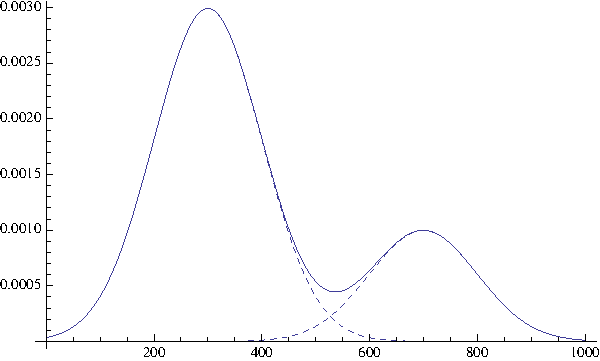
\includegraphics[scale=0.75]{mixture}
\end{center}
\caption{Example distribution, this figure does not necessarily match the data; the probability being female is essentially the cumulative distribution function of the female distribution.}
\end{figure}
\bigskip
\hrule 






\end{document}  
